\documentclass[]{article}
\usepackage[a4paper,top=3cm,bottom=2.5cm,left=2.5cm,
            right=2cm,marginparwidth=1.75cm,
            headheight=5pt]{geometry}
\usepackage[T5]{fontenc}
\usepackage[utf8]{inputenc}
\usepackage[document]{}
\usepackage[english]{babel}
\usepackage[unicode]{hyperref}
\usepackage{amsmath}
\usepackage{setspace}
\usepackage{graphicx}
\usepackage{caption}
\usepackage{subcaption}
\usepackage{tcolorbox}
\usepackage{listings}
\usepackage{hyperref}
\usepackage{xcolor}
\usepackage{longtable}
\usepackage{titlesec}
\usepackage{floatrow}
\usepackage[nottoc]{tocbibind}
\usepackage{mdframed}
\usepackage{amsmath}
\usepackage{amssymb}
\usepackage{tgbonum}
\usepackage{type1cm}
\usepackage{indentfirst}
\usepackage{lettrine}
\usepackage{colortbl}
\usepackage{fancyhdr}
\usepackage{wrapfig}
\usepackage{lastpage}
\usepackage{url}
\addto\captionsenglish{
  \renewcommand{\contentsname}{Table of Contents}%
  \renewcommand{\listfigurename}{Danh sách ảnh}%
  \renewcommand{\listtablename}{Danh sách bảng}%
  \renewcommand{\figurename}{Figure}
  \renewcommand{\tablename}{Table}
}
\pagestyle{fancy}
\fancyhf{}
\rhead{Intro to Machine Learning}
\lhead{\color{cyan}Google Data Analytics by Coursera}
\lfoot{Page \thepage /\pageref{LastPage}}
\renewcommand{\footrulewidth}{0.4pt}
\setlength{\parindent}{1.5em}
\setlength{\parskip}{1cm}
\renewcommand{\baselinestretch}{1.5}
\newmdenv[linecolor=black,skipabove=\topsep,skipbelow=\topsep,
leftmargin=2.5cm,rightmargin=2.5cm,
innerleftmargin=5cm,innerrightmargin=5cm]{mybox}
\usepackage{multicol}
\usepackage{indentfirst}
\usepackage{color}
\usepackage{tikz}
\graphicspath{{Figures/}} 
\usepackage{lipsum}
\usetikzlibrary{calc}
\setlength{\columnseprule}{2pt}
\def\columnseprulecolor{\color{black}}
\def\maru#1{\textcircled{\scriptsize#1}}

\usepackage[backend=biber, style=numeric]{biblatex}
\addbibresource{refs.bib} % Tải tệp references.bib
\defbibheading{mybibintoc}{\section{Tài liệu tham khảo}}


\begin{document}

% Bìa trang
\begin{titlepage}
  \begin{tikzpicture}[remember picture,overlay,inner sep=0,outer sep=0]
    \draw[blue!70!black,line width=4pt] ([xshift=-1.5cm,yshift=-2cm]current page.north east) coordinate (A)--([xshift=2cm,yshift=-2cm]current page.north west) coordinate(B)--([xshift=2cm,yshift=2cm]current page.south west) coordinate (C)--([xshift=-1.5cm,yshift=2cm]current page.south east) coordinate(D)--cycle;

    \draw ([yshift=0.5cm,xshift=-0.5cm]A)-- ([yshift=0.5cm,xshift=0.5cm]B)--
    ([yshift=-0.5cm,xshift=0.5cm]B) --([yshift=-0.5cm,xshift=-0.5cm]B)--([yshift=0.5cm,xshift=-0.5cm]C)--([yshift=0.5cm,xshift=0.5cm]C)--([yshift=-0.5cm,xshift=0.5cm]C)-- ([yshift=-0.5cm,xshift=-0.5cm]D)--([yshift=0.5cm,xshift=-0.5cm]D)--([yshift=0.5cm,xshift=0.5cm]D)--([yshift=-0.5cm,xshift=0.5cm]A)--([yshift=-0.5cm,xshift=-0.5cm]A)--([yshift=0.5cm,xshift=-0.5cm]A);


    \draw ([yshift=-0.3cm,xshift=0.3cm]A)-- ([yshift=-0.3cm,xshift=-0.3cm]B)--
    ([yshift=0.3cm,xshift=-0.3cm]B) --([yshift=0.3cm,xshift=0.3cm]B)--([yshift=-0.3cm,xshift=0.3cm]C)--([yshift=-0.3cm,xshift=-0.3cm]C)--([yshift=0.3cm,xshift=-0.3cm]C)-- ([yshift=0.3cm,xshift=0.3cm]D)--([yshift=-0.3cm,xshift=0.3cm]D)--([yshift=-0.3cm,xshift=-0.3cm]D)--([yshift=0.3cm,xshift=-0.3cm]A)--([yshift=0.3cm,xshift=0.3cm]A)--([yshift=-0.3cm,xshift=0.3cm]A);

  \end{tikzpicture}
  \newcommand{\HRule}{\rule{\linewidth}{0.5mm}}
  \center

  \textsc{\Large UNIVERSITY OF SCIENCE}\\[0.5cm]
  \textsc{\Large FACULTY OF INFORMATION TECHNOLOGY}\\[1cm]
  
\includegraphics[width=0.3\textwidth]{logo/KHTN.jpg}\\[1cm]

  \HRule \\[0.4cm]
  {\huge \bfseries GOOGLE DATA ANALYTICS} \\[0.4cm]
  {\large COURSERA}\\[0.1cm]
  \HRule \\[1.5cm]

  \centerline{\Large{\textbf{Triệu Nhật Minh — 21127112 — 21KHMT2}}}
  \vspace{2.5cm}
  \centerline{\large{\textit{Giảng viên hướng dẫn}}}
  \vspace{0.25cm}
  \centerline{\large{Bùi Duy Đăng}}
  \centerline{\large{Phạm Trọng Nghĩa}}
  \centerline{\large{Nguyễn Ngọc Đức}}
  \vspace{3cm}
  \centerline{\today}


  \vfill % Wipe blank space of the page.
\end{titlepage}

% Mục lục tự động
\setlength{\parskip}{.7em}
\tableofcontents
\newpage

% Table of Figures & Tables
\setlength{\parskip}{.5em}
%\listoffigures
%\listoftables
\newpage

% Bắt đầu nội dung

\section{Preface}
\subsection{About this course}
I am grateful for the opportunity to be one of the recipients of the 2022 Digital Talent Scholarship funded by NIC. This scholarship has enabled me to pursue my passion for data science and enhance my skills in this field. One of the remarkable features of this scholarship is that it is still active, which means I can continue to access various online courses and resources related to data. I have chosen to take the Google Data Analytics. In this report, I will share my opinions with the certificate and the course challenge.
\section{Certificate}
\subsection{Professional Certificate: Google Data Analytics by Coursera}
\begin{figure}[ht!]
  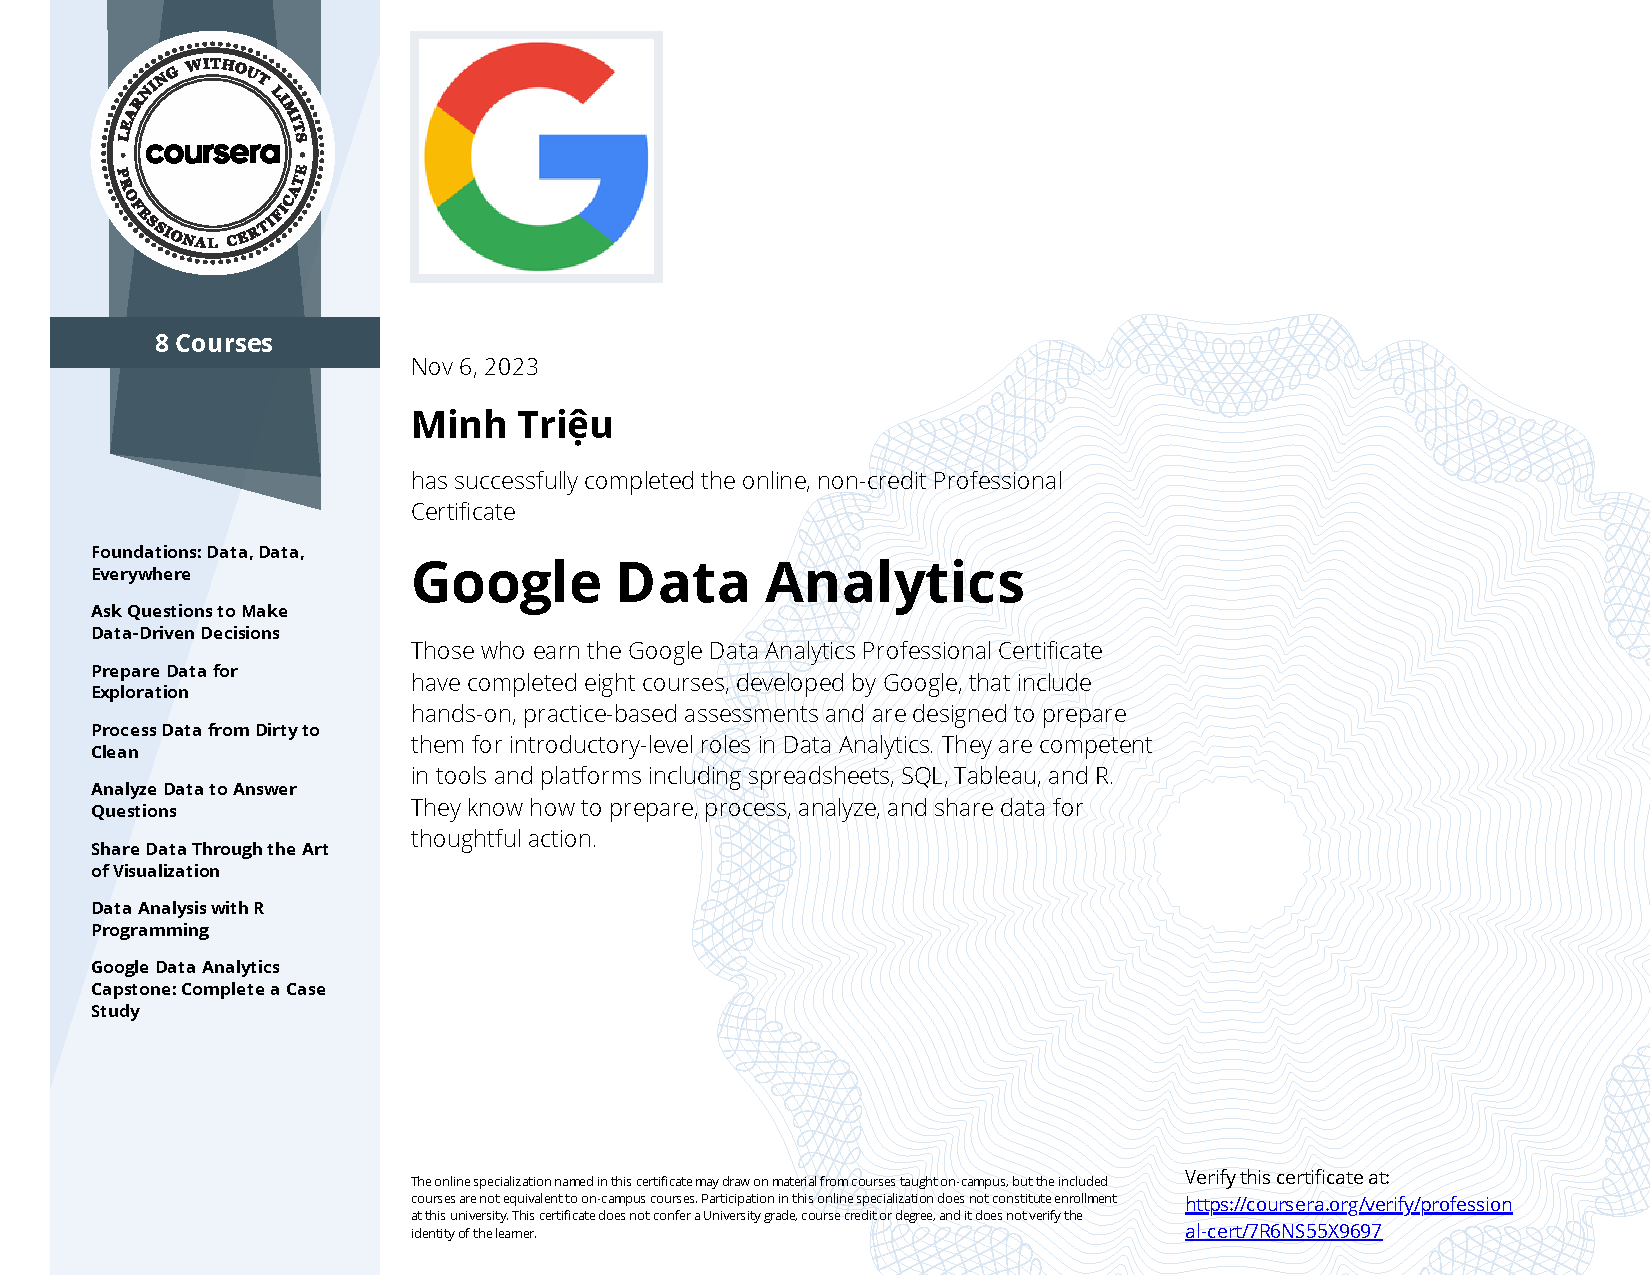
\includegraphics[width=0.2\textwidth]{certs/7R6NS55X9697.pdf}
  \caption{\href{https://www.coursera.org/account/accomplishments/specialization/certificate/7R6NS55X9697}{Verification}}
\end{figure}

\subsection{Enrollment date (8 courses)}
\begin{enumerate}
  \item \href{https://www.coursera.org/account/accomplishments/certificate/S9CWWMGFJAMM}{Foundations: Data, Data, Everywhere - 22nd October 2023}
  \item \href{https://www.coursera.org/account/accomplishments/certificate/ZA7TH6KEEEPB}{Ask Questions to Make Data-Driven Decisions - 24th October 2023}
  \item \href{https://www.coursera.org/account/accomplishments/certificate/B7PZ38G3U9XR}{Prepare Data for Exploration - 27th October 2023}
  \item \href{https://www.coursera.org/account/accomplishments/certificate/DYHS63889XUN}{Process Data from Dirty to Clean - 29th October 2023}
  \item \href{https://www.coursera.org/account/accomplishments/certificate/6478SYGTR4HF}{Analyze Data to Answer Questions - 5th November 2023}
  \item \href{https://www.coursera.org/account/accomplishments/certificate/8JULNPUM3GLC}{Share Data Through the Art of Visualization - 6th November 2023}
  \item \href{https://www.coursera.org/account/accomplishments/certificate/JPHDNMYYDJZ9}{Data Analysis with R Programming - 6th November 2023}
  \item \href{https://www.coursera.org/account/accomplishments/certificate/7TN58662AD9X}{Google Data Analytics Capstone: Complete a Case Study - 6th November 2023}
\end{enumerate}
Completion date of each course: On certificate verification link.

\section{Course 1: Foundations: Data, Data, Everywhere}
\begin{itemize}
  \item I have gained a lot of knowledge from the course. It has taught me how to turn data into insights and comprehend the data ecosystem. I have also learned how to use data to make informed business decisions.

  \item In module 2, I have developed my data analyst skills and practiced analytical thinking. I have learned how to define outcomes and how to measure them. I have also learned how to formulate good questions and communicate effectively with data.

  \item In module 3, I have followed the data life cycle and described the data analysis process. I have learned about the data analysis toolbox and how to apply different tools for different tasks. I have also learned how to clean, explore, analyze, and interpret data.

  \item In module 4, I have mastered spreadsheet basics and SQL. I have learned how to manipulate, query, and join data using spreadsheets and SQL. I have also learned how to plan a data visualization and select the right chart type for my data.

  \item In module 5, I have explored data analyst job opportunities and the importance of fair business decisions. I have learned how to prepare for a data analyst interview and showcase my portfolio. I have also learned how to avoid bias and ensure ethical use of data.

  \item This course has provided me with a solid foundation for becoming a data analyst. I have learned how to use data to make informed business decisions. I have also learned how to use spreadsheets and SQL for data analysis.

  \item About module challenges and course challenge, I find them very interesting and useful. They have helped me to practice my data analyst skills and apply what I have learned in the course. The instructor emphasizes the importance of asking questions and not making assumptions in data analysis work. He share a story about an analyst who initially struggled because he was afraid to ask questions, but improved significantly once he started doing so.
\end{itemize}
\section{Course 2: Ask Questions to Make Data-Driven Decisions}
\begin{itemize}
  \item
\end{itemize}
\section{Course 3: Prepare Data for Exploration}
\begin{itemize}
  \item
\end{itemize}
\section{Course 4: Process Data from Dirty to Clean}
\begin{itemize}
  \item
\end{itemize}
\section{Course 5: Analyze Data to Answer Questions}
\begin{itemize}
  \item
\end{itemize}
\section{Course 6: Share Data Through the Art of Visualization}
\begin{itemize}
  \item
\end{itemize}
\section{Course 7: Data Analysis with R Programming}
\begin{itemize}
  \item
\end{itemize}
\section{Course 8: Google Data Analytics Capstone: Complete a Case Study}
\begin{itemize}
  \item
\end{itemize}
\section{Conclusion}
\begin{itemize}
  \item
\end{itemize}
\end{document}